\documentclass[
]{jss}

\usepackage[utf8]{inputenc}

\providecommand{\tightlist}{%
  \setlength{\itemsep}{0pt}\setlength{\parskip}{0pt}}

\author{
Juan Pablo Marín Díaz\\Datasketch \And Jorge? Diego? Diego?\\The Nature Conservancy
}
\title{A Package for Estimating Carbon Capture and Biodiversity for Livestock
Farms in Colombia: \pkg{GanaderiaSostenible}}

\Plainauthor{Juan Pablo Marín Díaz, Jorge? Diego? Diego?}
\Plaintitle{A Package for Estimating Carbon Capture and Biodiversity for Livestock
Farms in Colombia: \pkg{GanaderiaSostenible}}
\Shorttitle{\pkg{GanaderiaSostenible}: Sustainable Livestock Farms}

\Abstract{
Open‐source software that is extensible and interactive is at the core
of appropriation of data driven methodologies for decision making.
Additionally, software interfaces that are easy to use for non-tech
users can provide a gateway for distribution of tools to be used by
non-specialists. In the contextos of sustainable farming practices and
with the objective to help farmers in Colombia the fight the climate
crisis we developed an interactive web based tool to estimate carbon
capture and biodiversity in farms through out all the colombian
territory with the most current estimations and projections for
different arrangements of land use. We describe de overall calculation
and the process to incorporate the results and projections and
distribute it through a user friendly interface.
}

\Keywords{Sustainable Livestock, Carbon Capture, Biodiversity, \proglang{R}}
\Plainkeywords{Sustainable Livestock, Carbon Capture, Biodiversity, R}

%% publication information
%% \Volume{50}
%% \Issue{9}
%% \Month{June}
%% \Year{2012}
%% \Submitdate{}
%% \Acceptdate{2012-06-04}

\Address{
    Juan Pablo Marín Díaz\\
  Datasketch\\
  Bogota, Colombia\\
  E-mail: \email{jpmarindiaz@datasketch.co}\\
  URL: \url{http://datasketch.co}\\~\\
      Jorge? Diego? Diego?\\
  The Nature Conservancy\\
  Bogota, Colombia\\
  E-mail: \email{this@tnc.org}\\
  URL: \url{http://tnc.org}\\~\\
  }


% Pandoc header

\usepackage{amsmath}

\begin{document}

\hypertarget{introduction}{%
\section{Introduction}\label{introduction}}

In an effort to provide decision makers and farmers with better tools to
fight the climate crisis. We have developed a web app to democratize
access to tools for carbon capture and biodiversity estimation in
Colombia.

The package and web application developed will allow farmers and other
interested parties to better plan land use implementations in farms for
sustainability. The web app allows users to estimate the carbon capture
in their farms and its biodiversity given their current location,
current land use and future implementations of coverage replacements
like silvopastoral, fencing or forests. Additionally the app provides
simulations and projections for land use planing.

In this article we describe the process of estimation and development of
the web app and the flow to package the solution as an open source R
package (\citet{RCoreTeam}) that covers the demands of R users in the
environmental field in Colombia, but also the needs of non-tech users
that access the computations through a user friendly web interface.

\hypertarget{background}{%
\section{Background}\label{background}}

In Colombia in particular the effects of global warming start to appear
INSERT MORE INFO HERE BACKED BY PUBLICATION \citet{Pending}. The charts
bellow show the annual median temperature has increased and the
reduction of annual rainfall.

\begin{figure}
\centering
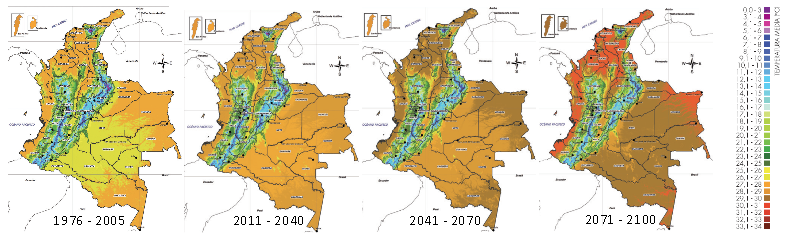
\includegraphics{figures/temperature.png}
\caption{Temperature increase in Colombia 1976 - 2100}
\end{figure}

\begin{figure}
\centering
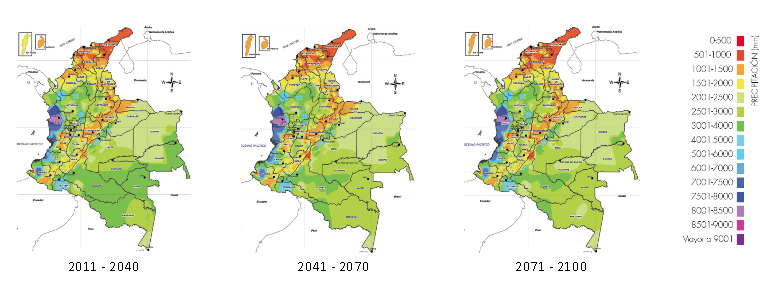
\includegraphics{figures/rainfall.png}
\caption{Rainfall decrease}
\end{figure}

Additionally, deforestation has played a big role. After the peace
agreement signed with FARC Rebels in 2016 there has been a considerable
increase in deforestation because of THIS AND THAT \citet{Pending}.

\begin{figure}
\centering
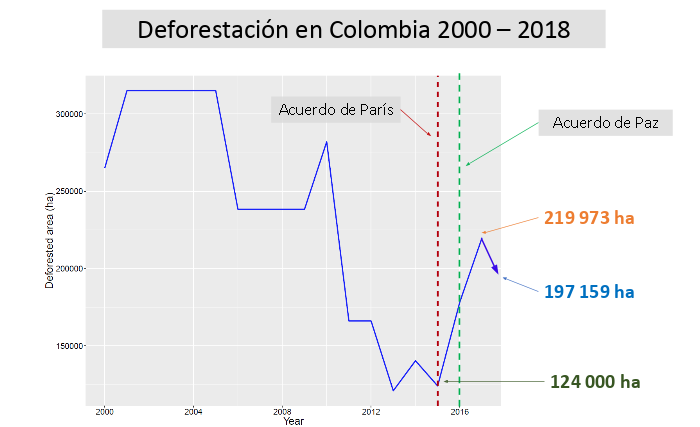
\includegraphics{figures/deforestation.png}
\caption{Deforestation in Colombia 2000 - 2018}
\end{figure}

\hypertarget{estimating-carbon-capture-in-colombia}{%
\subsection{Estimating Carbon Capture in
Colombia}\label{estimating-carbon-capture-in-colombia}}

Because of phtosythesis some organisms like plants capture carbon
dispersed in the atmosphere. This process helps reducing the
concentration of green house emissions, which are one of the major
causes of global warming \citet{Pending}.

INSERT DESCRIPTION ON THE THEORIES AND FORMULAS ON HOW EVERYTHING WAS
ALL CALCULATED, EXPLAIN CHART

\begin{figure}
\centering
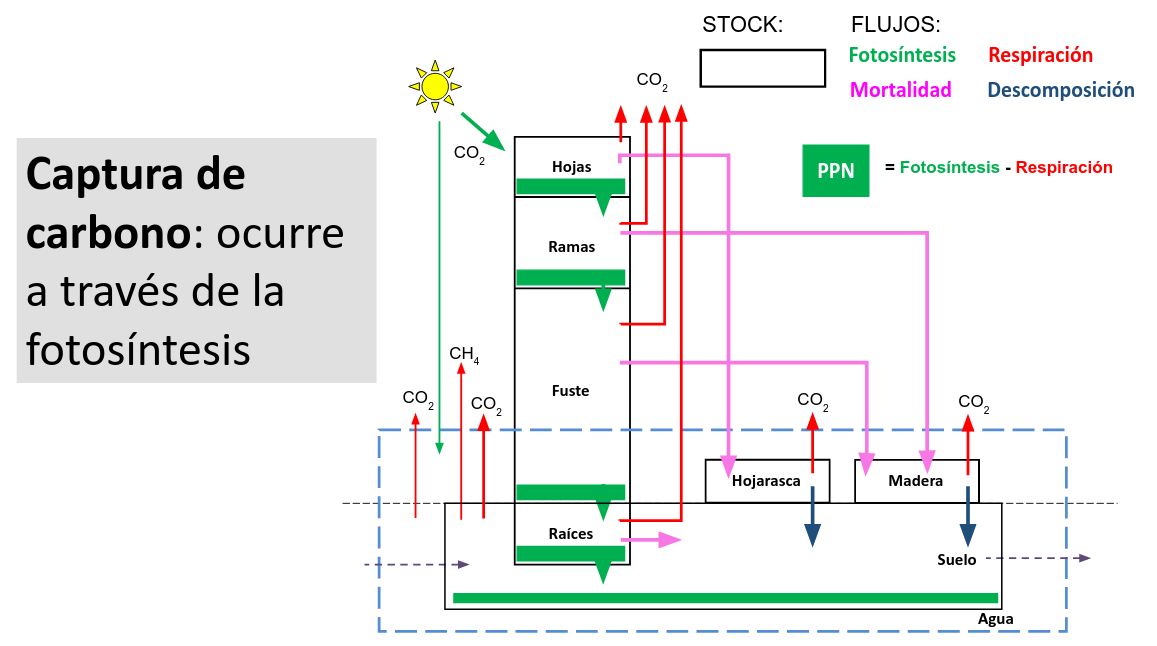
\includegraphics{figures/carbon-capture.png}
\caption{Carbon capture flow}
\end{figure}

\hypertarget{estimating-biodiversity}{%
\subsection{Estimating Biodiversity}\label{estimating-biodiversity}}

INSERT DESCRIPTION ON THE THEORIES AND FORMULAS ON HOW IT WAS ALL
CALCULATED

\hypertarget{emision-factors}{%
\subsection{Emision Factors}\label{emision-factors}}

INSERT DESCRIPTION ON THE THEORIES AND FORMULAS ON HOW IT WAS ALL
CALCULATED

\hypertarget{land-coverage}{%
\subsection{Land Coverage}\label{land-coverage}}

\begin{figure}
\centering
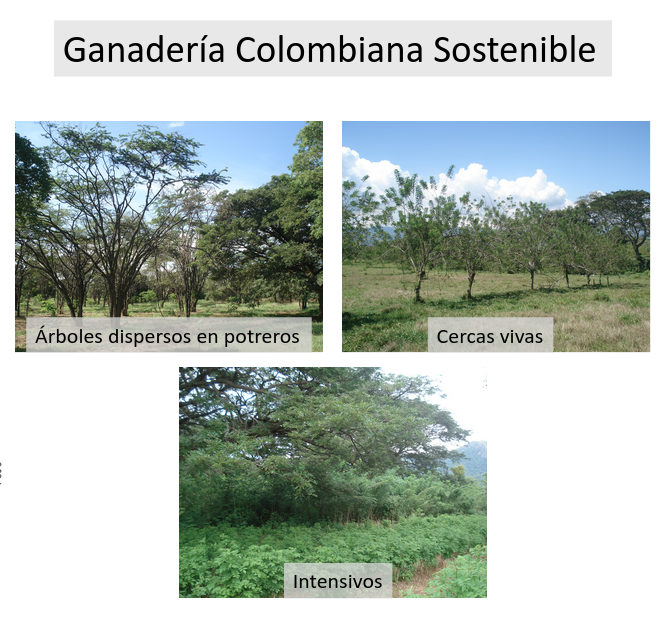
\includegraphics{figures/land-coverage.png}
\caption{Land coverage types}
\end{figure}

INSERT DESCRIPTION ON WHY THIS TYPES EXIST OR WHY THEY ARE IMPORTANT.

In livestock management in Colombia. There most common land uses
include:

\begin{itemize}
\tightlist
\item
  \textbf{Scattered trees}: It refers to native, naturalized or improved
  pastures in which trees are present in densities greater than 25 trees
  per hectare.
\item
  \textbf{Primary Forest}: Areas of mature forest that have not been
  intervened by humans in the last 30 years and whose use is strictly
  conserved. Activities such as timber extraction, hunting and
  agricultural practices are restricted in these areas.
\item
  \textbf{Bosque Secundario}: Forest areas in the process of natural
  regeneration in response to damage caused by human activities. Its use
  is of strict conservation and activities such as timber extraction,
  hunting and agricultural practices are restricted in these areas.
\item
  \textbf{Live fences}: Method to devide spaces or define boundaries in
  a property through planting trees, shrubs or palms as support instead
  of dead poles as support for barbed wire or smooth wire.
\item
  \textbf{Silvopastoral systems}: Arrangements in which there is a mix
  of trees, pastures and protein rich plants in a high density
  distribution.
\end{itemize}

\hypertarget{walkthrough}{%
\section{Walkthrough}\label{walkthrough}}

The design process revealed a layout using collapsible panels that
proved useful for interacting with the application in a single web ap
layout. From left to right, the users are taken through a journey of
exploration, from getting a graps of the basic concepts to get
simulation and projection results. The app leverage reactivity to auto
update custom

FALTA INCLUIR NÚMEROS EN LA IMAGEN DE ACUERDO DE ACUERDO A LA
CONFIRMACIÓN DE PASOS NECESARIOS PARA EL WALKTHROUGH

A step by step guide of the app components follow.

\begin{enumerate}
\def\labelenumi{\arabic{enumi}.}
\tightlist
\item
  Help module: Provides definitions and relevant links
\item
  Data Input: Users can input their location and the hectares for
  different land coverage types.
\item
  Results: This panel show the results, users can display information on
  carbon capture or biodiversity: 3.1 Carbon capture: It shows the total
  carbon captured captured and it's equivalence with relatable numbers
  for non-specialized users in automobile emisions per year.
  Additionally the results are shown with a stacked visualization chart
  for each land coverage type. 3.2 Biodiversity: The estimated number of
  bird species present in the farm for the given region and land usage
  is shown to the user
\item
  Advanced results: A simulation or projection for up to 20 years is
  visualized to show future estimates of carbon capture for each land
  coverage type.
\end{enumerate}

\begin{figure}
\centering
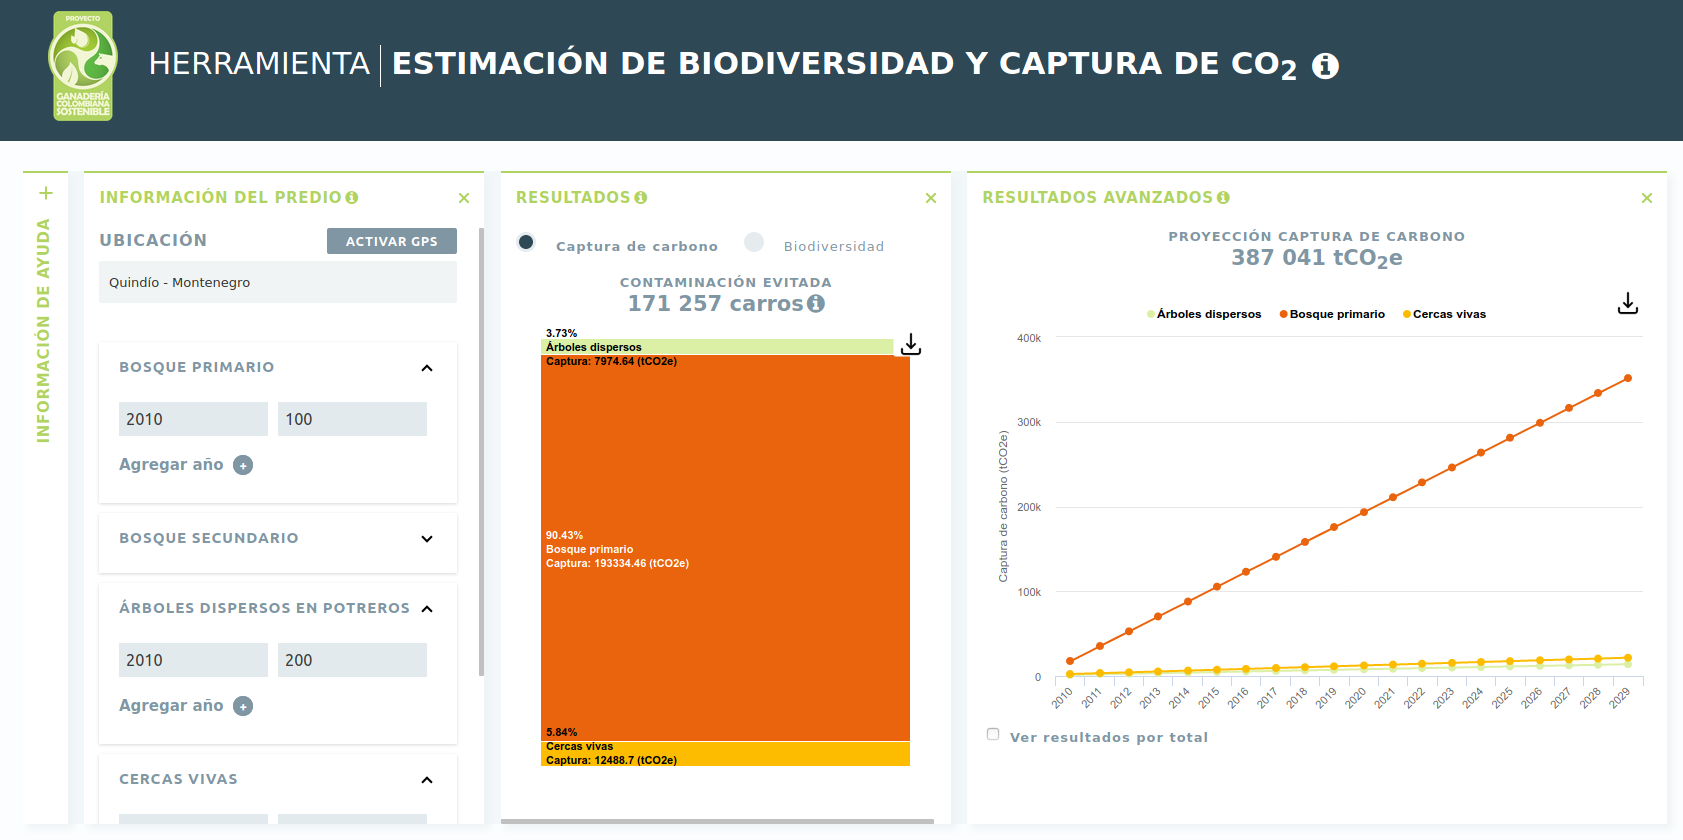
\includegraphics{figures/app.png}
\caption{Walktrhough of the application}
\end{figure}

\hypertarget{development}{%
\section{Development}\label{development}}

The purpose of the platform developed is to:

\begin{enumerate}
\def\labelenumi{\arabic{enumi}.}
\tightlist
\item
  Estimate carbon capture in colombian farms
\item
  Estimate Biodiversity present in farms
\item
  Simulate the effect of carbon capture and biodiversity for different
  implementation of land coverage types
\end{enumerate}

The first version of this tool involved a series of excel files with
different formats. For portability and appropriation reasons there is a
need make the implementation available to a wider audience.

Reproducible and accesible results play a big role in the appropriation
of data driven tools for decision makers and practitioners in
environmental the environmental field This is why we decided to launch a
paclkaged solution for farmers and researchers in researchers in
Colombia to have access to the most up to date estimates on carbon
capture and biodiversity present in colombian farms through out all the
territory. These estimates vary from region to region and according to
the land coverage types as described in the previous section.

To this end we used and R package that encompasses a web app using the
Shiny framework \citet{Chang2015}. This set up provides an appropiate
way not only to open up estimations and calculations to the research
community for different regions in Colombia, but also to deliver a
simple solution for non-tech users to interact with the platform. To
this end we went through a design process which led to the following
considerations for the web app:

\begin{itemize}
\tightlist
\item
  Single page app
\item
  Modular solution with collapsable panels
\item
  Informative landing page with summaries and relevant links
\end{itemize}

To achieve this a couple of new developments within the Shiny framework
where introduced:

\begin{itemize}
\tightlist
\item
  Implementation and adjustments to a package to lay out Shiny apps as
  collapsible panels.
\item
  Introduction of new shiny widgets for searching.
\end{itemize}

\hypertarget{reproducible-research}{%
\subsection{Reproducible Research}\label{reproducible-research}}

When we talk about being able to re-do our data analysis we must ensure
that the data structure is the same. To this end, several data sources
where standarized so we could have every input compatible with farm
locations which is one of the primary user inputs. Farm locations are
given by the user at the municipality level in Colombia, each
municipality in turn is mapped to the corresponding geographic regions
that correspond to available estimations of carbon capture and bird
species taken from multiple sources.

With this standarizations the package provides funcions that translate
locations and areas for each coverage type into carbon capture
estimations and projections to 20 years. When new data for carbon
capture becomes available, updating formulas can be done in
configuration files directly in the package, whenever possible,
hard-coded models are avoided to facilitate package maintenance.

\hypertarget{shiny-apps-in-a-software-package}{%
\subsection{Shiny apps in a software
package}\label{shiny-apps-in-a-software-package}}

As mentioned before Shiny allows to run R code in a webpage. Given that
we wanted to give an option for non-programmers to interact with the
package, we built a web app. In order to incorporate the web app to the
package one can simply put the code of the app online in a repository
and deploy it for users to interact. This approach is the easiest but it
is also difficult to maintain as the package code and the app do not
coexist. So in order to allow the two to coexist, but additionally to be
able to run the app from within the package on needs to include the web
app as a package function. You can run this function with
\texttt{runGanaderiaSostenible} which is a wrapper call to run Shiny
with the code for the app stored in the \texttt{inst/} folder of the
package.

To improve usability of the web app custom widgets where developed. The
inputSearch widget was adapted from an experimental package. This widget
binds a new input to the Shiny framework wich custom javascript code.
Additionally custom HTML components where included into the shiny layout
dependency to accomodate the large number of components.

New components and input controls where introduced:

\begin{itemize}
\tightlist
\item
  Custom search input
\item
  Collapsible boxes controls
\item
  Year and hectares dynamic inputs combo
\end{itemize}

\hypertarget{landing-page}{%
\subsection{Landing page}\label{landing-page}}

The landing page uses a static site generator implemented in the Go
language, called Hugo. It contains basic information about the project
and is available at: \url{http://datasketch.github.io/landing-gcs}

\hypertarget{further-work}{%
\section{Further work}\label{further-work}}

To extend the package, one would need to calibrate the models again
given data updates on carbon captures estimations. Re-calibrations of
the model amount to changing parameters in a configuration file with in
the package.

For the biodiversity estimation, only bird species where taken into
account, note that the species estimations are limited to XXXXX regions
covering XXXXX of the national territory. Future versions of this pakage
cound incorporate other estimates.

\hypertarget{acknowledgments}{%
\section{Acknowledgments}\label{acknowledgments}}

WHO SHOULD WE ACKNOWLEDGE?

\bibliography{bibliography.bib}


\end{document}

